% =====================================================================
%  Öğretici: İlk TikZ çiziminiz
% ---------------------------------------------------------------------
%  "%" ile başlayan satırlar yorumdur; derleyici onları okumaz.
%  Bu belgeyi adım adım değiştirin ve her seferinde "Derle" düğmesine
%  basarak sonucu sağdaki önizlemede görün.
% =====================================================================

% "standalone" sınıfı, sayfayı çizimin boyutuna göre kırpar.
% "tikz" seçeneği her tikzpicture ortamını ayrı bir sayfa yapar;
% "border=8pt" ise çizimin çevresine 8 puntoluk boşluk bırakır.
\documentclass[tikz,border=8pt]{standalone}

% TikZ paketini yüklüyoruz. Bütün çizim komutları bu paketten gelir.
\usepackage{tikz}

\begin{document}

% Her çizim bir tikzpicture ortamının içinde yazılır.
% Köşeli parantezdeki seçenekler tüm çizime uygulanır:
% "scale=1" ölçek, "line width" ise varsayılan çizgi kalınlığıdır.
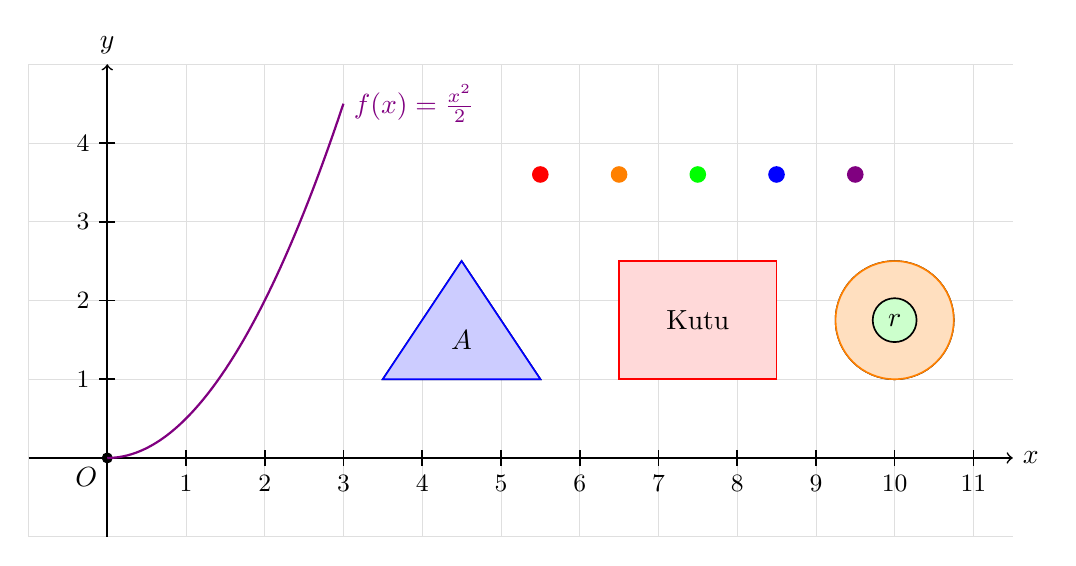
\begin{tikzpicture}[scale=1, line width=0.6pt]

  % -------------------------------------------------------------------
  % 1) KOORDİNATLAR
  % -------------------------------------------------------------------
  % TikZ'de bir nokta (x,y) biçiminde yazılır; birim varsayılan olarak
  % 1 santimetredir. (0,0) başlangıç noktasıdır.
  %
  % Önce açık gri bir kareli zemin çizelim: (-1,-1) köşesinden
  % (11.5,5) köşesine kadar, 1 birim aralıklarla.
  \draw[step=1, gray!25, very thin] (-1,-1) grid (11.5,5);

  % Eksenler: "->" seçeneği çizginin ucuna ok koyar.
  % "node[right] {$x$}" ise çizginin sonuna bir etiket ekler.
  \draw[->] (-1,0) -- (11.5,0) node[right] {$x$};
  \draw[->] (0,-1) -- (0,5) node[above] {$y$};

  % -------------------------------------------------------------------
  % 2) \draw İLE ÇİZGİ VE ŞEKİLLER
  % -------------------------------------------------------------------
  % "--" iki noktayı düz bir çizgiyle birleştirir.
  % "cycle" ise yolu başladığı noktaya geri kapatır (üçgen oldu!).
  \draw (3.5,1) -- (5.5,1) -- (4.5,2.5) -- cycle;

  % Dikdörtgen: karşılıklı iki köşesini vermek yeterli.
  \draw (6.5,1) rectangle (8.5,2.5);

  % Çember: merkez noktası ve yarıçap.
  \draw (10,1.75) circle (0.75);

  % -------------------------------------------------------------------
  % 3) RENKLER
  % -------------------------------------------------------------------
  % \filldraw hem çizer hem boyar. Aynı şekilleri bu kez renkli çizelim:
  % çizgi rengi için "draw=renk", iç dolgu için "fill=renk" yazılır.
  % "blue!20" mavinin %20'si, geri kalanı beyaz demektir (açık mavi).
  % Hazır renklerden bazıları: red, blue, green, orange, violet, gray.
  \filldraw[draw=blue, fill=blue!20] (3.5,1) -- (5.5,1) -- (4.5,2.5) -- cycle;
  \filldraw[draw=red, fill=red!15] (6.5,1) rectangle (8.5,2.5);
  \filldraw[draw=orange, fill=orange!25] (10,1.75) circle (0.75);

  % -------------------------------------------------------------------
  % 4) \node İLE YAZI EKLEMEK
  % -------------------------------------------------------------------
  % \node, belirtilen konuma bir yazı (veya kutu) yerleştirir.
  % Matematik ifadeleri her zamanki gibi $...$ içine yazılır.
  \node at (4.5,1.5) {$A$};
  \node at (7.5,1.75) {Kutu};

  % Seçeneklerle düğümü süsleyebilirsiniz: "draw" çerçeve çizer,
  % "circle" yuvarlak yapar, "fill" ise içini boyar.
  \node[draw, circle, fill=green!20] at (10,1.75) {$r$};

  % "above", "below", "left", "right" yazıyı noktanın yanına kaydırır.
  % Küçük dolu bir nokta koyup yanına etiket yazalım:
  \fill (0,0) circle (2pt) node[below left] {$O$};

  % -------------------------------------------------------------------
  % 5) DÖNGÜ: \foreach
  % -------------------------------------------------------------------
  % Aynı komutu birçok kez yazmak yerine döngü kullanın.
  % \i sırasıyla 1, 2, ..., 11 değerlerini alır; her biri için
  % x ekseninde küçük bir çentik ve altına sayısı çizilir.
  \foreach \i in {1,...,11} {
    \draw (\i,0.1) -- (\i,-0.1) node[below] {\small $\i$};
  }

  % Aynı şeyi y ekseni için yapalım.
  \foreach \j in {1,...,4} {
    \draw (0.1,\j) -- (-0.1,\j) node[left] {\small $\j$};
  }

  % Döngüyle renkli noktalar: renk adını da döngüden alabilirsiniz.
  \foreach \x/\renk in {1/red, 2/orange, 3/green, 4/blue, 5/violet} {
    \fill[\renk] (\x+4.5,3.6) circle (3pt);
  }

  % -------------------------------------------------------------------
  % 6) BASİT BİR FONKSİYON GRAFİĞİ
  % -------------------------------------------------------------------
  % "plot" komutu bir fonksiyonu çizer:
  %   domain=0:3      -> x değerleri 0 ile 3 arasında
  %   samples=50      -> 50 nokta hesaplanır (daha çok nokta = daha pürüzsüz)
  %   smooth          -> noktaları yumuşak bir eğriyle birleştirir
  %   variable=\x     -> değişkenin adı \x
  % ({\x}, {...}) ise her nokta için (x, f(x)) çiftidir.
  % Burada f(x) = 0.5 * x^2 parabolünü çiziyoruz.
  \draw[domain=0:3, samples=50, smooth, variable=\x, thick, violet]
    plot ({\x}, {0.5*\x*\x})
    node[right] {$f(x)=\frac{x^2}{2}$};

  % -------------------------------------------------------------------
  % SIRA SİZDE!
  % -------------------------------------------------------------------
  % - Üçgenin rengini "blue" yerine "red" yapıp yeniden derleyin.
  % - Çemberin yarıçapını 0.75 yerine 1 yapın.
  % - Parabolün formülünü {0.5*\x*\x} yerine {sin(\x r)} yaparak
  %   sinüs eğrisi çizin ("r", açının radyan olduğunu söyler).
  % Bir hata yaparsanız Derleme günlüğü size satır numarasını gösterir.

\end{tikzpicture}

\end{document}
